\subsection{Validazione e Collaudo}

\subsubsection{Divisione oraria}
La seguente tabella rappresenta la distribuzione oraria dei ruoli per ogni componente del gruppo:
{
\rowcolors{2}{grigetto}{white}
\renewcommand{\arraystretch}{2}
\begin{longtable}[h!] { C{4cm} C{1cm} C{1cm} C{1cm} C{1cm} C{1cm} C{1cm} C{3cm}}
\caption{Tabella della divisione oraria di Validazione e Collaudo}\\
\rowcolor{darkblue}

\textcolor{white}{\textbf{Membro del gruppo}} & 
\textcolor{white}{\textbf{RE}} & 
\textcolor{white}{\textbf{AM}} & 
\textcolor{white}{\textbf{AN}} & 
\textcolor{white}{\textbf{PT}} & 
\textcolor{white}{\textbf{PR}} &
\textcolor{white}{\textbf{VE}} &
\textcolor{white}{\textbf{Ore complessive}}\\	
\endhead
        
\MC{}                     &  - &  - &  7 &  - &  4 &  8 &  19 \\
\LD{}                     &  - &  4 &  - &  5 &  - & 10 &  19 \\
\CE{}                     &  5 &  - &  - &  - &  6 & 12 &  23 \\ 
\SE{}                     &  - &  - &  - &  6 &  5 &  9 &  20 \\
\PF{}                     &  6 &  - &  - &  - &  7 &  8 &  21 \\
\DF{}                     &  - &  6 &  - &  - &  9 &  6 &  21 \\
\BR{}                     &  - &  5 &  - &  - &  6 & 10 &  21 \\
\AT{}                     &  - &  - &  4 & 10 &  - &  7 &  21 \\
\textbf{Ore totali ruolo} & 11 & 15 & 11 & 21 & 37 & 70 & 165 \\
		
\end{longtable}
}


La suddivisione delle ore svolte da ciascun componente del gruppo per ogni ruolo viene rappresentata nel seguente istogramma:
\begin{figure}[h!]
	\centering
	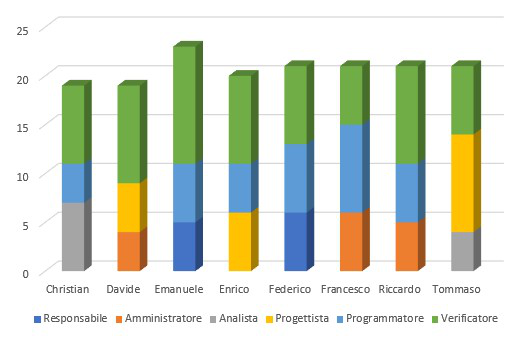
\includegraphics{Sezioni/Istogrammi/IstogrammaValidazione.png}
	\caption{Disposizione ore per ruolo di ciascun componente della fase di Validazione e Collaudo}
\end{figure}

\clearpage

\subsubsection{Costo risultante}
La seguente tabella rappresenta rappresenta per ogni ruolo le ore totali investite e il corrispondente costo in euro:
{
\rowcolors{2}{grigetto}{white}
\renewcommand{\arraystretch}{2}
\begin{longtable}{ C{3cm} C{2cm} C{4cm}}
\caption{Tabella del costo risultante di Validazione e Collaudo}\\
\rowcolor{darkblue}

\textcolor{white}{\textbf{Ruolo}} & 
\textcolor{white}{\textbf{Totale ore}} & 
\textcolor{white}{\textbf{Costo ruolo (in \euro{})}}\\	
\endhead
        
Responsabile    &  11 &  330 \\
Amministratore  &  15 &  300 \\
Analista        &  11 &  275 \\
Progettista     &  21 &  462 \\
Programmatore   &  37 &  555 \\
Verificatore    &  70 & 1050 \\
\textbf{Totale} & 169 & 2972 \\
	
\end{longtable}
}

La quantità di ore totali per ciascun ruolo viene rappresentata nel seguente areogramma:
\begin{figure}[h!]
	\centering
	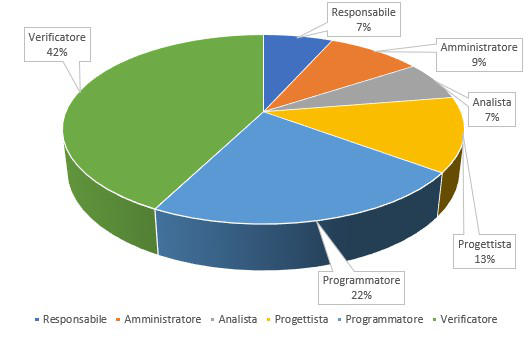
\includegraphics{Sezioni/Aerogrammi/AerogrammaValidazione.png}
	\caption{Suddivisione ore per ruolo della fase di Validazione e Collaudo}
\end{figure}
